\chapter[Equiprobable Outcomes]{Equiprobable Outcomes and Combinatorics}

The simplest probabilistic scenario is one where the sample space $\Omega$ is finite and all the possible outcomes are equally likely.
In such cases, computing the probability of an event amounts to counting the number of outcomes comprising this event and dividing the sum by the total number of elements contained in the sample space.
This situation was first explored in Section~\ref{section:FiniteSampleSpaces}, with an explicit formula for computing probabilities appearing in \eqref{equation:ProbEquiProbableOutcomes}.

While counting outcomes may appear intuitively straightforward, it is in many circumstances a daunting task.
For instance, consider the number of distinct subsets of the integers $\{ 1, 2, \ldots, n \}$ that do not contain two consecutive integers.
This number is equal to
\begin{equation*}
\frac{ \phi^{n+2} - (1 - \phi)^{n+2} }{ \sqrt{5} } ,
\end{equation*}
where $\phi = (1 + \sqrt{5}) / 2$ is the \emph{golden ratio}.
This somewhat surprising result can be obtained iteratively through the \emph{Fibonacci} recurrence relation, and it attests of the fact that counting may at times be challenging.
Calculating the number of ways that certain patterns can be formed is part of the field of \emph{combinatorics}. \index{Combinatorics}
In this chapter, we introduce useful counting techniques that can be applied to situations pertinent to probability.


\section{The Counting Principle}

The counting principle is a guiding rule for computing the number of elements in a cartesian product.
Suppose that $S$ and $T$ are finite sets with $m$ and $n$ elements, respectively.
The cartesian product of $S$ and $T$ is given by
\begin{equation*}
S \times T = \{ (x, y) | x \in S \text{ and } y \in T \} .
\end{equation*}
The number of elements in the cartesian product $S \times T$ is equal to $m n$.
This is illustrated in the figure below.

\begin{center}
\begin{psfrags}
\psfrag{1}[c]{$1$}
\psfrag{2}[c]{$2$}
\psfrag{3}[c]{$3$}
\psfrag{a}[c]{$a$}
\psfrag{b}[c]{$b$}
\includegraphics[height=6.495cm]{Figures/4Chapter/countingprinciple}
\end{psfrags}
\end{center}

\begin{example}
Consider an experiment consisting of flipping a coin and rolling a die.
There are two possibilities for the coin, heads or tales, and the die has six faces.
The total number of outcomes for this experiment is $2 \times 6 = 12$.
That is, there are twelve different ways to flip a coin and roll a die.
\end{example}

The counting principle can be extended to computing the number of elements in the cartesian product of multiple sets.
Consider the finite sets $S_1, S_2, \ldots, S_r$ and their cartesian product
\begin{equation*}
S_1 \times S_2 \times \cdots \times S_r
= \left\{ (s_1, s_2, \ldots, s_r) | s_p \in S_p \right\} .
\end{equation*}
If we denote the cardinality of $S_p$ by $n_p = | S_p |$, then the number of distinct ordered $r$-tuples of the form $(s_1, s_2, \ldots, s_r)$ is $n = n_1 n_2 \cdots n_r$.

\begin{example}[Sampling with Replacement and Ordering]
An urn contains $n$ balls numbered one through $n$.
A ball is drawn from the urn, and its number is recorded on an ordered list.
The ball is then replaced in the urn.
This procedure is repeated $k$ times.
We wish to compute the number of possible sequences that results from this experiment.
There are $k$ drawings and $n$ possibilities per drawing.
Using the counting principle, we conclude that the number of distinct sequences is $n^k$.

\begin{center}
\begin{psfrags}
\psfrag{1}[c]{$1$}
\psfrag{2}[c]{$2$}
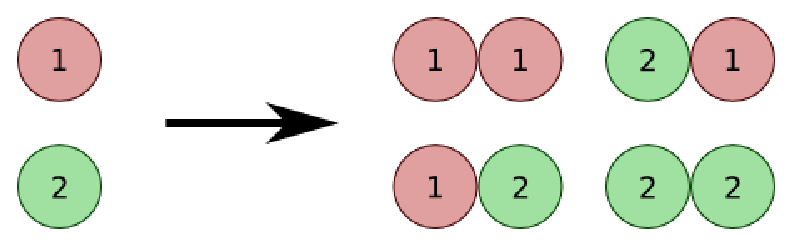
\includegraphics[height=1.91cm]{Figures/4Chapter/sequences}
\end{psfrags}
\end{center}
\end{example}

\begin{example}
The power set of $S$, denoted by $2^S$, is the set of all subsets of $S$.
In set theory, $2^S$ represents the set of all functions from $S$ to $\{ 0, 1\}$.
By identifying a function in $2^S$ with the corresponding preimage of one, we obtain a bijection between $2^S$ and the subsets of $S$.
In particular, each function in $2^S$ is the characteristic function of a subset of $S$.

Suppose that $S$ is finite with $n = |S|$ elements.
For every element of $S$, a characteristic function in $2^S$ is either zero or one.
There are therefore $2^n$ distinct characteristic functions from $S$ to $\{ 0, 1\}$.
Hence, the number of distinct subsets of $S$ is given by $2^n$.

\begin{center}
\begin{psfrags}
\psfrag{1}[c]{$1$}
\psfrag{2}[c]{$2$}
\psfrag{3}[c]{$3$}
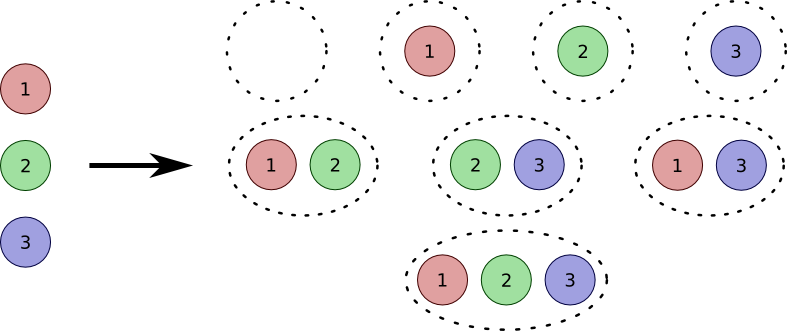
\includegraphics[height=4.965cm]{Figures/4Chapter/powerset}
\end{psfrags}
\end{center}
\end{example}


\section{Permutations}

Again, consider the integer set $S = \{ 1, 2, \ldots, n \}$.
A \emph{permutation} of $S$ is an ordered arrangement of its elements, a list without repetitions. \index{Permutation}
The number of permutations of $S$ can be computed as follows.
First, there are $n$ distinct possibilities for the first item in the list.
The number of possibilities for the second item is $n-1$, namely all the integers in $S$ except the first element in the list.
Similarly, the number of distinct possibilities for the $m$th item is $n - m + 1$.
This pattern continues until all the elements in $S$ are recorded.
Summarizing, we find that the total number of permutations of $S$ is $n$ \emph{factorial}, \index{Factorial}
\begin{equation*}
n! = n (n-1) \cdots 1 .
\end{equation*}

\begin{example}
We wish to compute the number of permutations of $S = \{ 1, 2, 3 \}$.
Since the set $S$ possesses three elements, it has $3! = 6$ different permutations.
They can be written as $123, 132, 213, 231, 312, 321$.
\end{example}

\begin{center}
\begin{psfrags}
\psfrag{1}[c]{$1$}
\psfrag{2}[c]{$2$}
\psfrag{3}[c]{$3$}
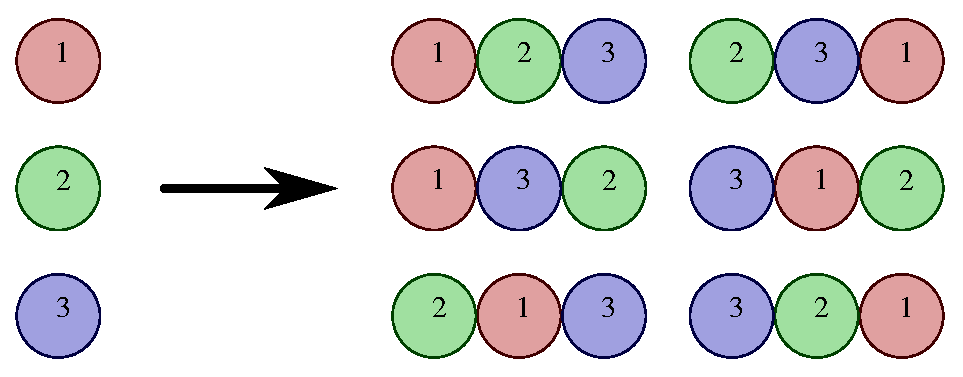
\includegraphics[height=3.06cm]{Figures/4Chapter/permutation}
\end{psfrags}
\end{center}


\subsection{Stirling's Formula*}

The number $n!$ grows very rapidly as a function of $n$.
A good approximation for $n!$ when $n$ is large is given by \emph{Stirling's formula}, \index{Stirling's formula}
\begin{equation*}
n! \sim n^n e^{-n} \sqrt{ 2 \pi n}
\end{equation*}
as $n \rightarrow \infty$.
The notation $a_n \sim b_n$ signifies that the ratio $a_n / b_n \rightarrow 1$ as $n \rightarrow \infty$.


\subsection{$k$-Permutations}

Suppose that we rank only $k$ elements out of the set $S = \{ 1, 2, \ldots, n \}$, where $k \leq n$.
We wish to count the number of distinct $k$-permutations of $S$.
Following our previous argument, we can choose one of $n$ elements to be the first item listed, one of $(n-1)$ elements for the second item, and so on.
The procedure terminates when $k$ items have been recorded.
The number of possible sequences is then given by
\begin{equation*}
\frac{n!}{(n-k)!} = n (n-1) \cdots (n-k+1) .
\end{equation*}

\begin{example}
A recently formed music group has four original songs they can play.
They are asked to perform two songs at a music festival.
We wish to compute the number of song arrangements the group can offer in concert.
Abstractly, this is equivalent to computing the number of $2$-permutations of four songs.
Thus, the number of distinct arrangements is ${4!}/{2!} = 12$.
\end{example}

\begin{center}
\begin{psfrags}
\psfrag{1}[c]{$1$}
\psfrag{2}[c]{$2$}
\psfrag{3}[c]{$3$}
\psfrag{4}[c]{$4$}
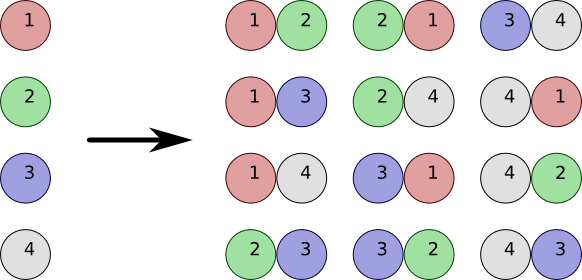
\includegraphics[height=4.215cm]{Figures/4Chapter/kpermutation}
\end{psfrags}
\end{center}

\begin{example}[Sampling without Replacement, with  Ordering]
An urn contains $n$ balls numbered one through $n$.
A ball is picked from the urn, and its number is recorded on an ordered list.
The ball is not replaced in the urn.
This procedure is repeated until $k$ balls are selected from the urn, where $k \leq n$.
We wish to compute the number of possible sequences that results from this experiment.
The number of possibilities is equivalent to the number of $k$-permutations of $n$ elements, which is given by $n! / (n-k)!$.
\end{example}


\section{Combinations}

Consider the integer set $S = \{ 1, 2, \ldots, n \}$.
A \emph{combination} is a subset of $S$. \index{Combination}
We emphasize that a combination differs from a permutation in that elements in a combination have no specific ordering.
The $2$-element subsets of $S = \{ 1, 2, 3, 4 \}$ are
\begin{equation*}
\{ 1, 2 \}, \{ 1, 3 \}, \{ 1, 4 \}, \{ 2, 3 \}, \{ 2, 4 \}, \{ 3, 4 \} ,
\end{equation*}
whereas the $2$-permutations of $S$ are more numerous with
\begin{equation*}
\begin{split}
&( 1, 2 ), ( 1, 3 ), ( 1, 4 ), ( 2, 1 ), ( 2, 3 ), ( 2, 4 ), \\
&( 3, 1 ), ( 3, 2 ), ( 3, 4 ), ( 4, 1 ), ( 4, 2 ), ( 4, 3 ) .
\end{split}
\end{equation*}
There are therefore fewer $2$-element subsets of $S$ than $2$-permutations of $S$.

\begin{center}
\begin{psfrags}
\psfrag{1}[c]{$1$}
\psfrag{2}[c]{$2$}
\psfrag{3}[c]{$3$}
\psfrag{4}[c]{$4$}
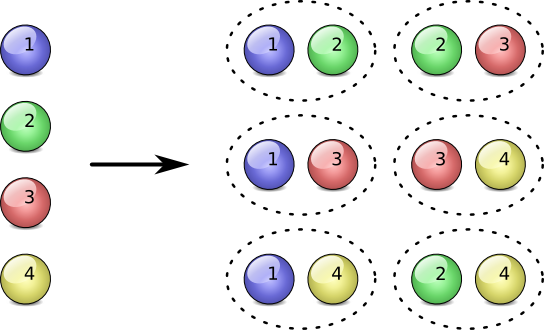
\includegraphics[height=4.95cm]{Figures/4Chapter/combination}
\end{psfrags}
\end{center}

We can compute the number of $k$-element combinations of $S = \{ 1, 2, \ldots, n \}$ as follows.
First, we note that a $k$-permutation can be formed by first selecting $k$ objects from $S$ and then ordering them.
There are $k!$ distinct ways of ordering $k$ objects.
The number of $k$-permutations must then equal the number of $k$-element combinations multiplied by $k!$.
Since the total number of $k$-permutations of $S$ is $n! / (n-k)!$, the number of $k$-element combinations is found to be
\begin{equation*}
\binom{n}{k} = \frac{n!}{k! (n-k)!} = \frac{ n (n-1) \cdots (n-k+1) }{ k! } .
\end{equation*}
This expression is termed a \emph{binomial coefficient}. \index{Binomial coefficient}
Observe that selecting a $k$-element subset of $S$ is equivalent to choosing the $n-k$ elements that belong to its complement.
It follows that
\begin{equation*}
\binom{n}{k} = \binom{n}{n-k} .
\end{equation*}

\begin{example}[Sampling without Replacement or Ordering]
An urn contains $n$ balls numbered one through $n$.
A ball is drawn from the urn and placed in a separate jar.
This process is repeated until the jar contains $k$ balls, where $k \leq n$.
We wish to compute the number of distinct combinations the jar can hold after the completion of this experiment.
Because there is no ordering in the jar, this amounts to counting the number of $k$-element subsets of a given $n$-element set, which is given by
\begin{equation*}
\binom{n}{k} = \frac{n!}{k! (n-k)!}.
\end{equation*}
\end{example}

Again, let $S = \{1, 2, \ldots, n\}$.
Since a combination is also a subset and the number of $k$-element combinations of $S$ is $\binom{n}{k}$, the sum of the binomial coefficients $\binom{n}{k}$ over all values of $k$ must be equal to the number of elements in the power set of $S$.
Thus, we get
\begin{equation*}
\sum_{k=0}^n \binom{n}{k} = 2^n .
\end{equation*}


\section{Partitions}

Abstractly, a combination is equivalent to partitioning a set into two subsets, one containing $k$ objects and the other containing the $n-k$ remaining objects.
In general, the set $S = \{ 1, 2, \ldots, n \}$ can be partitioned into $r$ subsets.
Let $n_1, n_2, \ldots, n_r$ be nonnegative integers such that
\begin{equation*}
\sum_{p = 1}^r n_p = n.
\end{equation*}
Consider the following iterative algorithm that leads to a \emph{partition} of $S$. \index{Partition}
First, we choose a subset of $n_1$ elements from $S$.
Having selected the first subset, we pick a second subset containing $n_2$ elements from the remaining $n - n_1$ elements.
We continue this procedure by successively choosing subsets of $n_p$ elements from the remaining $n - n_1 - \cdots - n_{p-1}$ elements, until no element remains.
This algorithm yields a partition of $S$ into $r$ subsets, with the $p$th subset containing exactly $n_p$ elements.

We wish to count the number of such partitions.
We know that there are $\binom{n}{n_1}$ ways to form the first subset.
Examining our algorithm, we see that there are exactly
\begin{equation*}
\binom{n - n_1 - \cdots - n_{p-1}}{n_p}
\end{equation*}
ways to form the $p$th subset.
Using the counting principle, the total number of partitions is then given by
\begin{equation*}
\binom{n}{n_1} \binom{n - n_1}{n_2}
\cdots \binom{n - n_1 - \cdots - n_{r-1}}{n_r},
\end{equation*}
which after simplification can be written as
\begin{equation*}
\binom{n}{n_1, n_2, \ldots, n_r}
= \frac{n!}{n_1! n_2! \cdots n_r!} .
\end{equation*}
This expression is called a \emph{multinomial coefficient}. \index{Multinomial coefficient}

\begin{example}
A die is rolled nine times.
We wish to compute the number of outcomes for which every odd number appears three times.
The number of distinct sequences in which one, three, and five each appear three times is equal to the number of partitions of $\{ 1, 2, \ldots, 9 \}$ into three subsets of size three, namely
\begin{equation*}
\frac{9!}{3! 3! 3!} = 1680 .
\end{equation*}
\end{example}

In the above analysis, we assume that the cardinality of each subset is fixed.
Suppose instead that we are interested in counting the number of ways to pick the cardinality of the subsets that form the partition. \index{Partition}
Specifically, we wish to compute the number of ways integers $n_1, n_2, \ldots, n_r$ can be selected such that every integer is nonnegative and
\begin{equation*}
\sum_{p = 1}^r n_p = n.
\end{equation*}
We can visualize the number of possible assignments as follows.
Picture $n$ balls space out on a straight line and consider $r-1$ vertical markers, each of which can be put between two consecutive balls, before the first ball, or after the last ball. 
For instance, if there are five balls and two markers then one possible assignment is illustrated below.

\begin{center}
\begin{psfrags}
\psfrag{1}[c]{$1$}
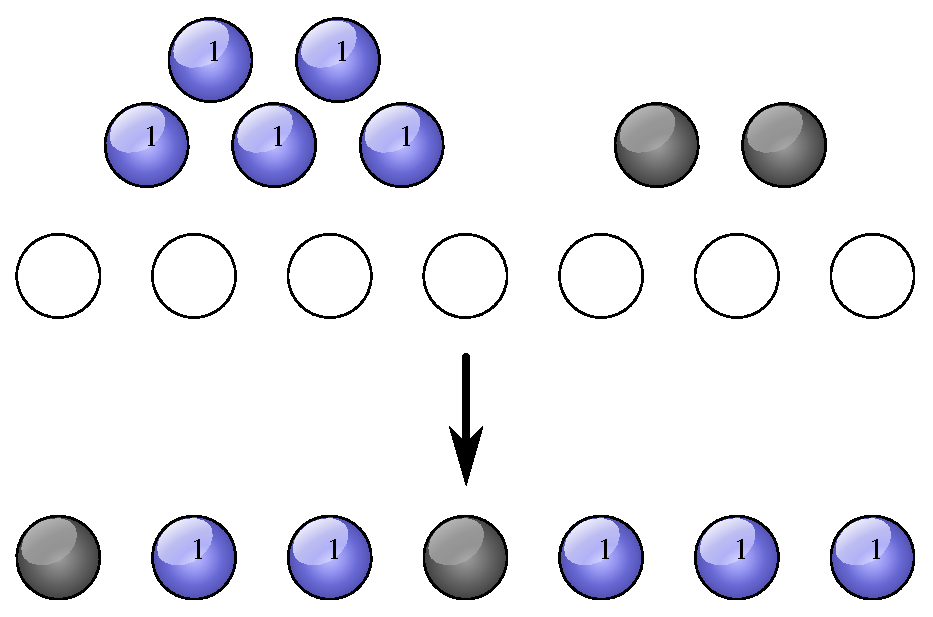
\includegraphics[height=5.28cm]{Figures/4Chapter/partitioning}
\end{psfrags}
\end{center}

The number of objects in the first subset corresponds to the number balls before the first marker.
Similarly, the number of objects in the $p$th subset is equal to the number of balls between the $p$th marker and the preceding one.
Finally, the number of objects in the last subset is simply the number of balls after the last marker.
The integer assignment associated with the figure above is
\begin{equation*}
(n_1, n_2, n_3) = (0,2,3).
\end{equation*}

\begin{center}
\begin{psfrags}
\psfrag{1}[c]{$1$}
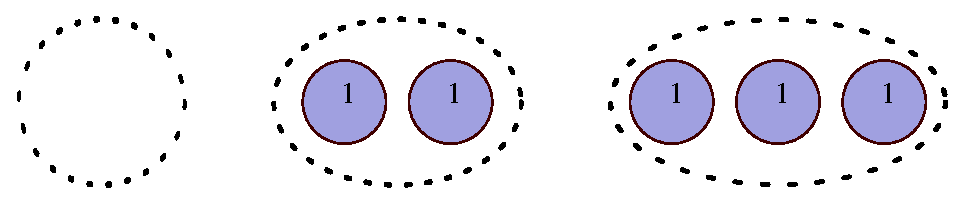
\includegraphics[height=1.53cm]{Figures/4Chapter/partitioning2}
\end{psfrags}
\end{center}

In this scheme, two consecutive markers imply that the corresponding subset is empty.
There is a natural bijection between an integer assignment and the graphical representation depicted above.
To count the number of possible integer assignments, it suffices to calculate the number of ways to position the markers and the balls.
In particular, there are $n + r - 1$ positions, $n$ balls and $r - 1$ markers.
The number of ways to assign the markers is equal to the number of $n$-combinations of $n + r - 1$ elements,
\begin{equation*}
\binom{n + r - 1}{n} = \binom{n + r - 1}{r - 1} .
\end{equation*}

\begin{example}[Sampling with Replacement, without Ordering]
An urn contains $r$ balls numbered one through $r$.
A ball is drawn from the urn and its number is recorded.
The ball is then returned to the urn.
This procedure is repeated a total of $n$ times.
The outcome of this experiment is a table that contains the number of times each ball has come in sight.
We are interested in computing the number of distinct outcomes.
This is equivalent to counting the ways a set with $n$ elements can be partitioned into $r$ subsets.
The number of possible outcomes is therefore given by
\begin{equation*}
\binom{n + r - 1}{n} = \binom{n + r - 1}{r - 1} .
\end{equation*}
\end{example}


\section{Combinatorial Examples}

In this section, we present two applications of combinatorics to computing the probability of winning the lottery.

\begin{example}[Pick 3 Texas Lottery]
The Texas Lottery game ``Pick $3$'' is easy to play.
A player must pick three numbers from zero to nine, and choose how to play them: exact order or any order.
The Pick $3$ balls are drawn using three air-driven machines.
These machines use compressed air to mix and select each ball.

The probability of winning while playing the exact order is
\begin{equation*}
\frac{1}{10} \frac{1}{10} \frac{1}{10}
= \frac{1}{1000} .
\end{equation*}
The probability of winning while playing any order depends on the numbers selected.
If three distinct numbers are selected then the probability of winning is
\begin{equation*}
\frac{3!}{1000} = \frac{3}{500} .
\end{equation*}
If a number is repeated twice, the probability of winning is
\begin{equation*}
\frac{\binom{3}{2}}{1000} = \frac{3}{1000} .
\end{equation*}
While, if the same number is selected three times, the probability of winning becomes $1/1000$.
\end{example}

\begin{example}[Mega Millions Texas Lottery]
To play the Mega Millions game, a player must select five numbers from $1$ to $56$ in the upper white play area of the play board, and one Mega Ball number from $1$ to $46$ in the lower yellow play area of the play board.
All drawing equipment is stored in a secured on-site storage room.
Only authorized drawings department personnel have keys to the door.
Upon entry of the secured room to begin the drawing process, a lottery drawing specialist examines the security seal to determine if any unauthorized access has occurred.
For each drawing, the Lotto Texas balls are mixed by four acrylic mixing paddles rotating clockwise.
High speed is used for mixing and low speed for ball selection.
As each ball is selected, it rolls down a chute into an official number display area.
We wish to compute the probability of winning the Mega Millions Grand Prize, which require the correct selection of the five white balls plus the gold Mega ball.

The probability of winning the Mega Millions Grand Prize is
\begin{equation*}
\frac{1}{\binom{56}{5}} \frac{1}{46}
= \frac{51!5!}{56!} \frac{1}{46}
= \frac{1}{175 711 536} .
\end{equation*}
\end{example}

\begin{example}[Sinking Boat]
Six couples (twelve people total) are out at sea on a small sail boat.
Unfortunately, the boat hits an iceberg and starts sinking slowly.
Two Coast Guard boats, the Ibis and the Mako, come to the rescue of the passengers.
Each person must decide which of the two rescue boats to board.
What is the probability that no two people from a same couple end up on the Mako?

Suppose that all the passengers choose a rescue boat independently of one another.
For a given couple, the probability that the two members do not end up on the Mako is $3/4$.
Since couples act independently, the probability that no two people from a same couple are united on the Mako becomes $3^6/4^6$.
There are a total of $2^{12}$ possible arrangements of people on the Mako after the rescue operation, all equally likely.
Thus, there are only $729$ arrangements where no two members from a same couple board the Mako.
\end{example}

\begin{example}[The Locksmith Convention*]
A total of $n$ people are gathering to attend a two-day, secret locksmith convention.
As tradition dictates, every locksmith brings a lock and two keys to the convention.
At the opening ceremony, all the locksmiths sit around a large table, and they exchange a key to their own locks with the two members sitting immediately next to them.
The rules of the secret society stipulate that the conference can only continue on the second day if a working lock-and-key combination can be reconstituted.
If each locksmith decides to attend the second day of the convention with probability half, independently of others, what is the probability that the reunion can proceed on the second day?

Given that there are $n$ people on the first day, the number of arrangements on the second day is $2^n$, and they are all equally likely.
To find the probability that the reunion can proceed, it suffices to count the number of ways in which at least two people that were sitting next to each other during the opening ceremony are present.
Alternatively, we can compute the likelihood that this does not occur.
To solve this problem, we label the people attending the opening ceremony using integers one through $n$, according to their positions around the table.
We consider three situations that may occur on the second day for which the society's requirements are not met: member~$1$ is present, member~$n$ is present, and they are both absent from the conference.
If member~$1$ is present, then members~$2$ and $n$ cannot be there on the second day, and the number of possible non-qualifying arrangements is equal to the number of distinct subsets of the integers $\{3, 4,\ldots, n-1\}$ that do not contain consecutive integers.
This number can be deduced from the discussion at the beginning of this chapter, and is given by
\begin{equation*}
\frac{ \phi^{n-1} - (1 - \phi)^{n-1} }{ \sqrt{5} } .
\end{equation*}
By symmetry, the number of arrangements for which a lock-and-key combination cannot be reconstituted when member~$n$ shows up on the second day is
\begin{equation*}
\frac{ \phi^{n-1} - (1 - \phi)^{n-1} }{ \sqrt{5} } .
\end{equation*}
Finally, if both members~$1$ and $n$ are absent, then there are a total of
\begin{equation*}
\frac{ \phi^{n} - (1 - \phi)^{n} }{ \sqrt{5} }
\end{equation*}
combinations for which the meeting cannot proceed, as this is the number of distinct subsets of the integers $\{ 2, 3, \ldots, n-1 \}$ that do not contain consecutive integers.
Thus, the probability that the meeting can proceed is
\begin{equation*}
1 - \frac{ 2 \frac{ \phi^{n-1} - (1 - \phi)^{n-1} }{ \sqrt{5} }
+ \frac{ \phi^{n} - (1 - \phi)^{n} }{ \sqrt{5} } }{2^n} .
\end{equation*}
\end{example}

